\documentclass[border=6pt]{standalone}
% Shared preamble for web figures.  Each figure is a standalone .tex that
% \input's this file; scripts/make-figures.sh turns it into an SVG.
% Handouts pull the same file with \fig{Unit_X/<name>}.
\usepackage[T1]{fontenc}
\usepackage{helvet}
\renewcommand{\familydefault}{\sfdefault}
\renewcommand{\ttdefault}{pcr}  % Courier: a real Type 1 typewriter font
\usepackage{amsmath}
\usepackage{tikz}
\usetikzlibrary{arrows.meta,positioning,calc,shapes.symbols,shapes.geometric}

% Who makes the rules is the point of most diagrams in this book, so the
% colors mean the same thing everywhere: blue is a person, orange is the
% computer, green is an answer, pink is the human brain.
\definecolor{person}{HTML}{2C6FAE}
\definecolor{machine}{HTML}{D35400}
\definecolor{result}{HTML}{1E8449}
\definecolor{brainpink}{HTML}{C2185B}
\definecolor{ink}{HTML}{2C3E50}

\tikzset{
  doodle/.style={line width=1.5pt, line cap=round, line join=round, draw=ink},
  box/.style={draw, rounded corners=5pt, line width=1.1pt, align=center,
              inner sep=7pt, minimum height=1.0cm, font=\small},
  personbox/.style={box, draw=person, fill=person!10},
  machinebox/.style={box, draw=machine, fill=machine!10},
  resultbox/.style={box, draw=result, fill=result!10},
  plainbox/.style={box, draw=ink!70, fill=ink!4},
  flow/.style={-{Stealth[length=8pt]}, line width=1.4pt, draw=ink},
}

% A person (blue) and a robot head (orange) as small icons.
% \personicon{x}{y}{scale}   \roboticon{x}{y}{scale}
\newcommand{\personicon}[3]{%
  \begin{scope}[shift={(#1,#2)}, scale=#3]
    \fill[person] (0,0.62) circle (0.28);
    \fill[person, rounded corners=6pt] (-0.42,-0.55) rectangle (0.42,0.28);
  \end{scope}}
\newcommand{\roboticon}[3]{%
  \begin{scope}[shift={(#1,#2)}, scale=#3]
    \draw[machine, line width=1.2pt] (0,0.5) -- (0,0.72);
    \fill[machine] (0,0.78) circle (0.08);
    \draw[machine, line width=1.4pt, fill=machine!12, rounded corners=4pt] (-0.5,-0.45) rectangle (0.5,0.5);
    \fill[ink] (-0.2,0.12) circle (0.08);
    \fill[ink] (0.2,0.12) circle (0.08);
    \draw[ink, line width=1pt] (-0.22,-0.22) -- (0.22,-0.22);
  \end{scope}}

\begin{document}
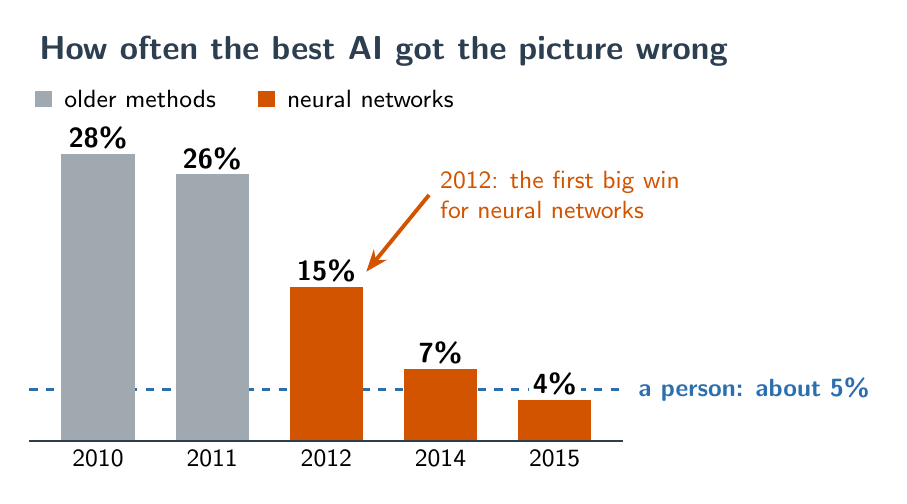
\begin{tikzpicture}[x=1.45cm, y=0.13cm]
% ImageNet contest (ILSVRC), top-5 error of the winning entry each year,
% rounded: 2010 28%, 2011 26%, 2012 AlexNet 15%, 2014 GoogLeNet 7%,
% 2015 ResNet 4%.  A person: about 5% (Karpathy's estimate).
\node[anchor=west, font=\large\bfseries, text=ink] at (-0.6,38) {How often the best AI got the picture wrong};
\fill[ink!45] (-0.55,32.6) rectangle (-0.4,34.2); \node[anchor=west, font=\small] at (-0.38,33.4) {older methods};
\fill[machine] (1.4,32.6) rectangle (1.55,34.2); \node[anchor=west, font=\small] at (1.57,33.4) {neural networks};
\draw[person, dashed, line width=1.3pt] (-0.6,5) -- (4.6,5);
\foreach \i/\yr/\v/\col in {0/2010/28/ink!45, 1/2011/26/ink!45, 2/2012/15/machine, 3/2014/7/machine, 4/2015/4/machine} {
  \fill[\col] (\i-0.32,0) rectangle (\i+0.32,\v);
  \node[above, font=\bfseries, fill=white, inner sep=1.5pt] at (\i,\v) {\v\%};
  \node[below, font=\small] at (\i,0) {\yr};
}
\draw[ink, line width=0.8pt] (-0.6,0) -- (4.6,0);
\node[anchor=west, font=\small\bfseries, text=person] at (4.65,5) {a person: about 5\%};
\draw[flow, draw=machine] (2.9,24) node[anchor=west, font=\small, text=machine, align=left] {2012: the first big win\\for neural networks} -- (2.35,16.5);
\end{tikzpicture}
\end{document}
